
\chapter{Minimalizuj wpływ ognisk}
\label{rule4-fire}

\section{Wpływ ognisk}

W przypadku rozważania wpływu wywieranego przez palenie ognisk na środowisko nie zajmujemy się zagrożeniem pożarowym. Bezpieczeństwo ognisk jest koniecznym punktem wyjścia, bez którego nie powinniśmy w ogóle zaczynać rozważań o wpływie tychże na środowisko. 

We wszelkich poniższych przykładach zakładamy zatem, że ogniska rozpalane są w sposób bezpieczny, w miejscu do tego przeznaczonym lub wyznaczonym, poza okresami zagrożenia pożarowego i przy spełnieniu wszelkich innych prawnych aspektów z tym związanych.

\subsection{Wypalanie}

Pierwszym, bezpośrednim i najbardziej widocznym wpływem wywieranym przez ogniska jest wypalenie gleby i powstanie nowego ,,miejsca ogniskowego''. Wszelkie rośliny rosnące na powierzchni gleby pod samym ogniskiem oraz w jego najbliższym otoczeniu zostają spalone. Wysoka temperatura ponadto zabija żywe organizmy żyjące w glebie - bezkręgowce, mikroorganizmy, rośliny, grzyby, bakterie -  nawet do głębokości kilkudziesięciu centymetrów, w zależności od wielkości ogniska oraz czasu jego palenia.
Biologicznie czynna, powierzchniowa warstwa gleby zostaje w ten sposób wyjałowiona. Powrót organizmów żywych i ich ponowną kolonizację tego obszaru ogranicza zaś zmiana odczynu gleby.

\begin{minipage}{0.5\textwidth}

\begin{figure}[!hb]
	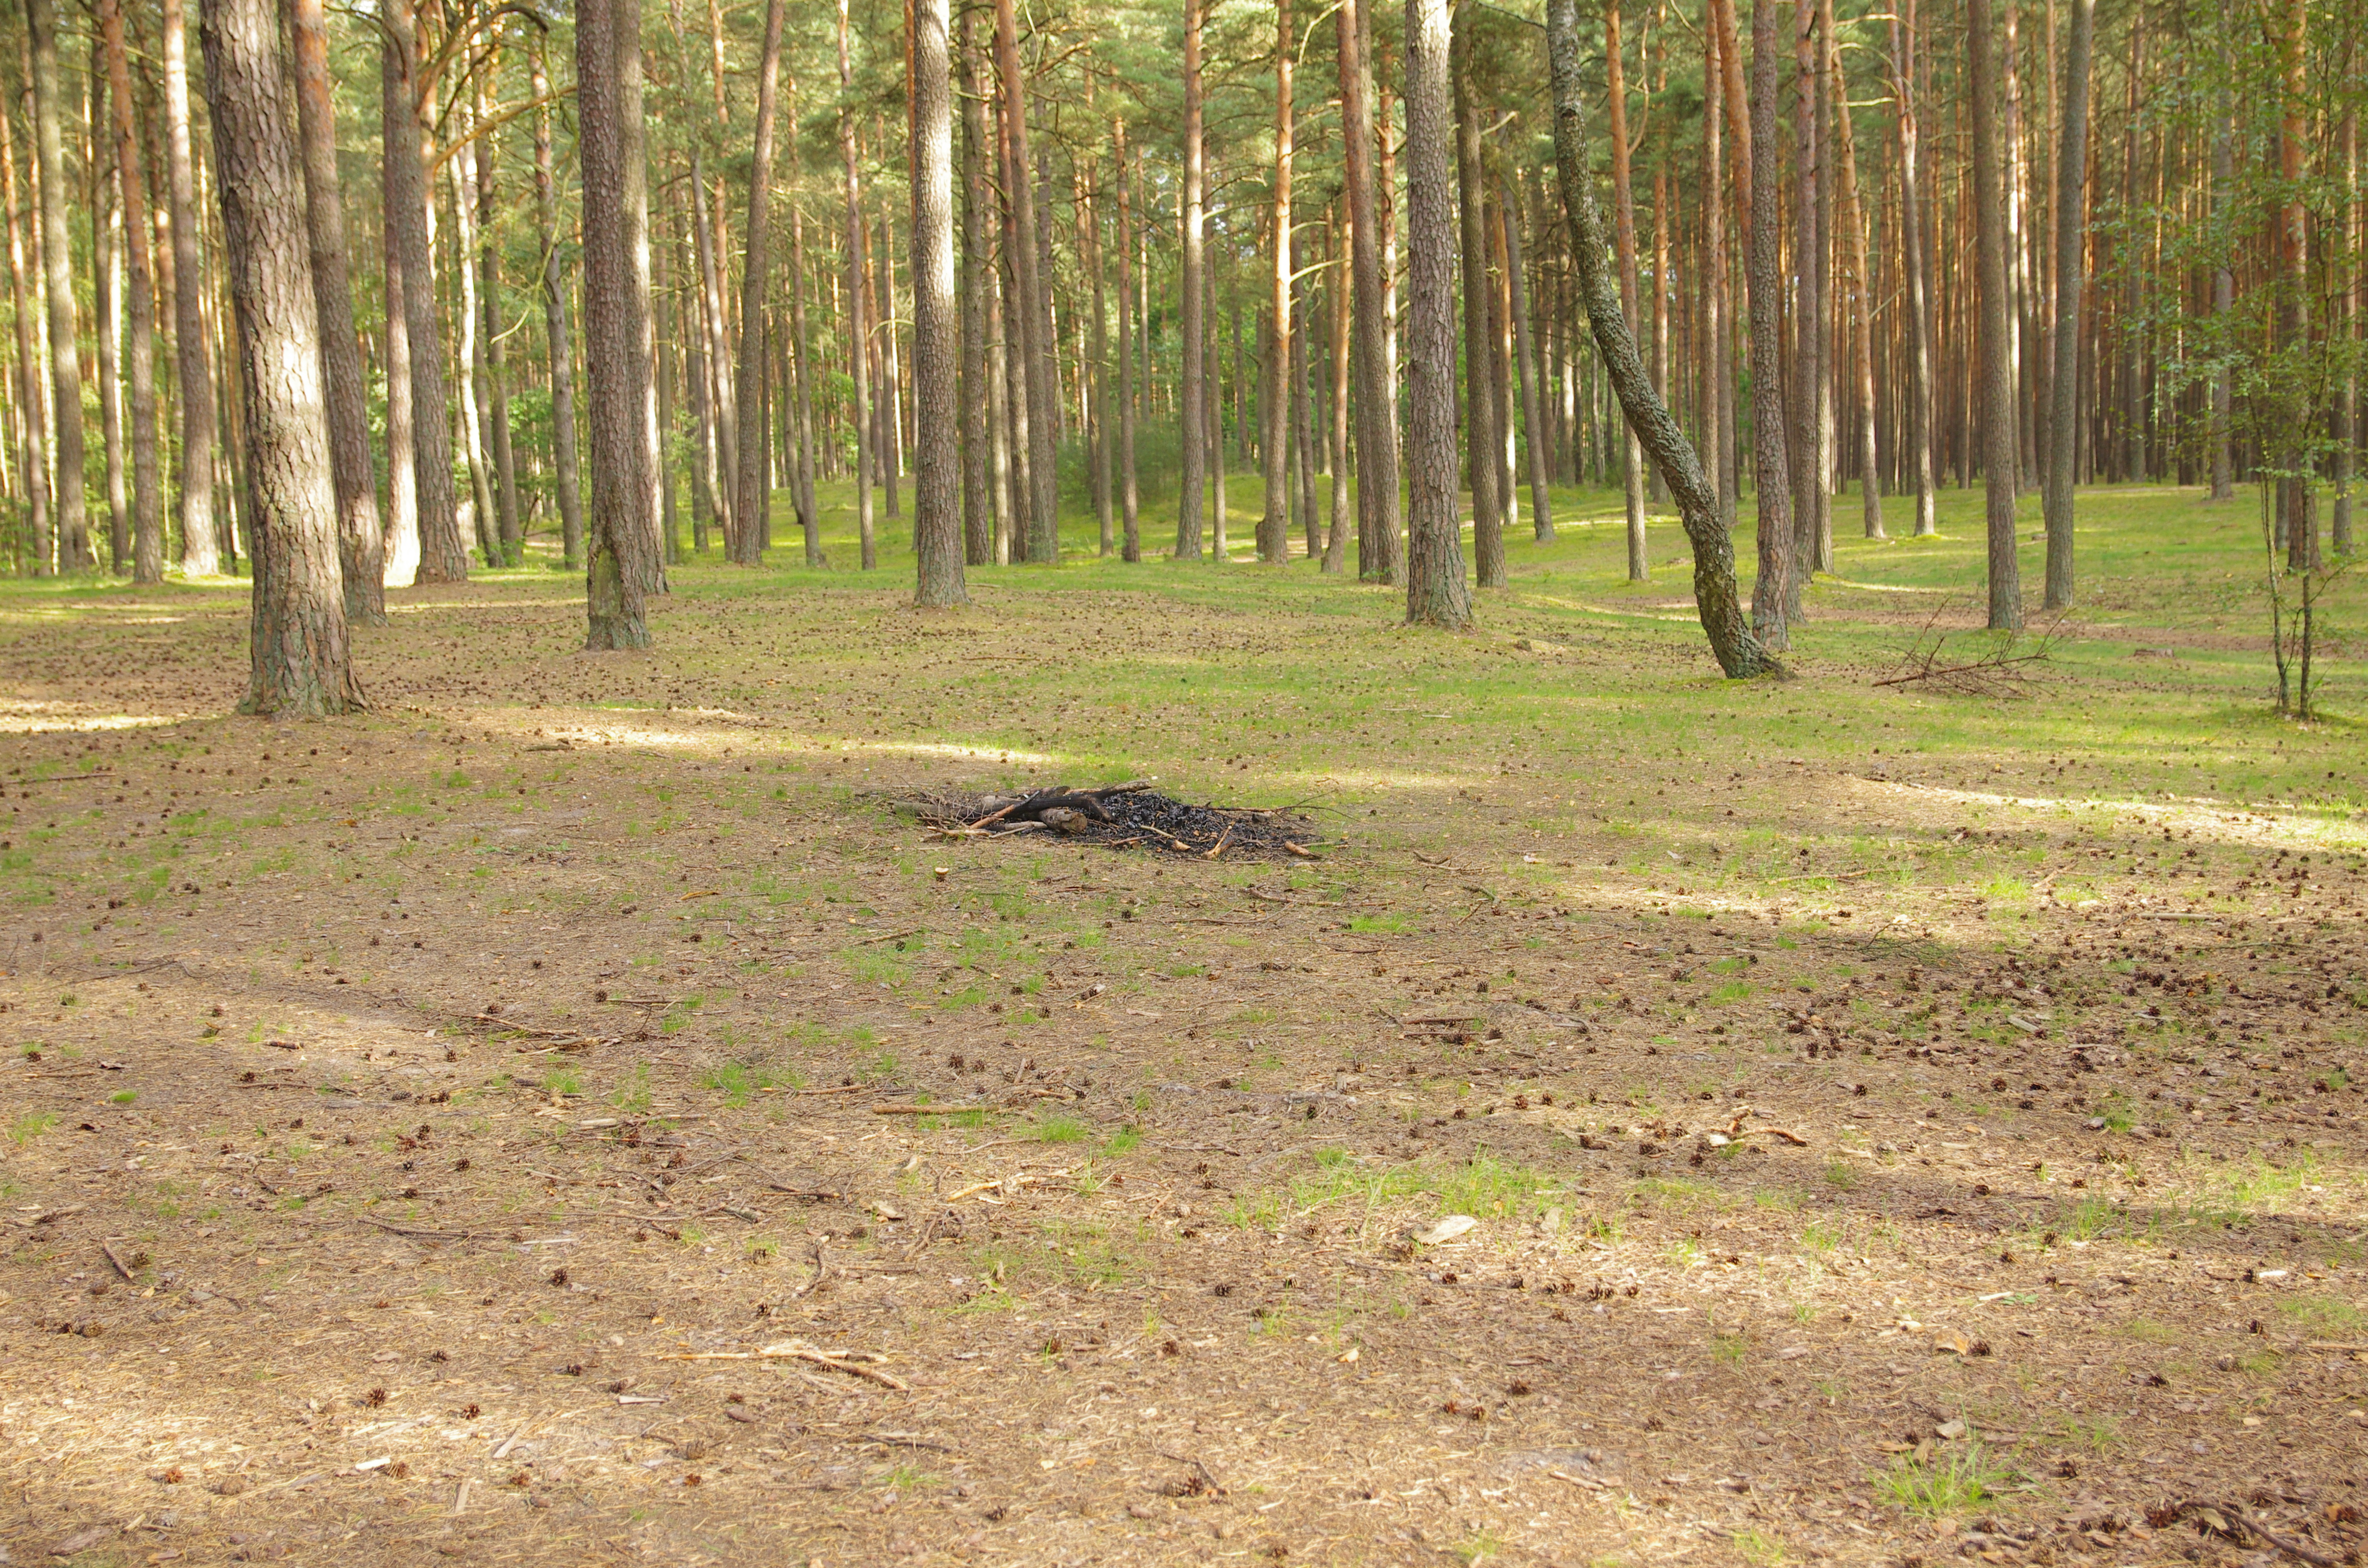
\includegraphics[width=0.5\textwidth]{obrazy/ognisko}
	\caption[Wypalone ognisko.]{Pozostałości ogniska w miejscu, w którym wcześniej ognisk nie było. Taki wypalony ślad pozostawiony bez rekultywacji zabliźniać się będzie kilka lat. Pozostałości obozu harcerskiego w miejscowości Trzebciny, Bory Tucholskie.}
\end{figure}

\end{minipage}

\subsection{Zmiana odczynu gleby}



\subsection{Dym}

\subsection{Drewno}

\section{Po co nam ogniska oraz alternatywy}

\section{Minimalizacja wpływu ognisk}

\subsection{Skupienie, rozproszenie}